section{マルチラベル推定}
レスキュー犬訓練データセットのマルチラベル推定を行なった.動画で見たデータセットの前半70\%を学習、後半30\%を評価に用いた.
モデル毎にそれぞれチューニングを行い,モデル内で最も精度の良いものを示す.
各表ではクラス毎の精度と全体を合計しての精度をPrecision(適合性),Recall(再現率),Jaccard係数で示している.
なお,Jaccard係数とは\[\tfrac{TP}{FP+FN+TP}\]で表され,PrecisionとRecallの両者についてF尺度と比較してより厳格な値が求まる.
レスキュー犬の行動分類にあたり,PrecisionとRecallを共に重視するためにこの係数を採用した.
よって,本研究ではJaccard係数がより大きいモデルは精度がより良いと表現する.

\subsection{静止画像からのマルチクラス推定}
静止画像からのマルチクラス推定では,ImageNetで学習したVGG16のpretrained modelを用いてのfinetuningを行なった.
推定精度を表~\ref{still_result}に示す.
%表~\ref{cyberdataset_label}と照らしあわせると,データ数の少ないものは精度が低い傾向にある.
%eatクラス,runクラスが特にその傾向を反映している.傾向とは異なるものとして,

eatクラス,runクラスが特に精度が低く,データ数の少なさと関係していると考察できる.
データ数が少ないにも関わらずPrecisionの高いshakeクラス,反対にデータ数が十分にも関わらず精度の低いsniffクラスからは,図~\ref{cyberdataset_img}に示したように画像特徴の取りやすさ、取りにくさに依存していることが確認できる.
\begin{table}[tb]
 \centering
 \caption{静止画像を用いたVGG16のfinetuning結果}\label{still_result}
 \scalebox{0.85}[0.85]{
  \begin{tabular}{|l||c|c|c|c|c|c|c|c|c|c|c|c|}
   \hline \hline
   クラス   & \rotatebox{90}{bark}& \rotatebox{90}{cling}&\rotatebox{90}{command}& \rotatebox{90}{eat}&\rotatebox{90}{handler}& \rotatebox{90}{run}&\rotatebox{90}{victim}& \rotatebox{90}{shake}& \rotatebox{90}{sniff}& \rotatebox{90}{stop}& \rotatebox{90}{walk} & \rotatebox{90}{全体}\\ \hline
%Precision & 0.626& 0.112& 0.046& 0.23& 0.249& nan& 0.347& 0.896& 0.0& 0.777& 0.602&  0.576 \\ \hline
%Recall    & 0.363& 0.227& 0.067& 0.031& 0.027& 0.0& 0.38& 0.3& 0.0& 0.704& 0.753&  0.605 \\ \hline
%Jaccard   & 0.299& 0.081& 0.028& 0.028& 0.025& 0.0& 0.222& 0.29& 0.0& 0.586& 0.503&  0.418 \\ \hline
   % seven80_6fps_still_bc-32_lr-0_sr-5_sp-30

Precision & 0.475& 0.148& 0.0& 0.377& 0.611& nan& 0.37& nan& nan& 0.74& 0.636&  0.565 \\ \hline
Recall    & 0.333& 0.108& 0.0& 0.025& 0.059& 0.0& 0.313& 0.0& 0.0& 0.742& 0.72&  0.656 \\ \hline
Jaccard   & 0.244& 0.066& 0.0& 0.024& 0.057& 0.0& 0.204& 0.0& 0.0& 0.588& 0.51&  0.436 \\ \hline
   % seven80_6fps_still_bc-32_lr-6_sr-5_sp-30
  \end{tabular}
 }
\end{table}

\subsection{optical flow画像からのマルチクラス推定}
optical flow画像からのマルチクラス推定では,静止画像からのマルチラベル推定と同じようにImageNetで学習したVGG16のpretrained modelを用いてのfinetuningを行なった.
推定精度を表~\ref{optic_result}に示す.

静止画像と比較して,shakeクラス,stopクラスなどの動き特徴の現れやすそうなクラスの精度が高くなることを期待していたが,それらを含め全体的に精度が下がった.
画像特徴が失われたため,推定が困難になった様子がうかがえる.
\begin{table}[tb]
 \centering
 \caption{optical flow画像を用いたVGG16のfinetuning結果}\label{optic_result}
 \scalebox{0.86}[0.86]{
  \begin{tabular}{|l||c|c|c|c|c|c|c|c|c|c|c|c|}
   \hline \hline
   クラス   & \rotatebox{90}{bark}& \rotatebox{90}{cling}&\rotatebox{90}{command}& \rotatebox{90}{eat}&\rotatebox{90}{handler}& \rotatebox{90}{run}&\rotatebox{90}{victim}& \rotatebox{90}{shake}& \rotatebox{90}{sniff}& \rotatebox{90}{stop}& \rotatebox{90}{walk} & \rotatebox{90}{全体}\\ \hline
%   Precision & 0.54& 0.027& 0.017& 0.183& 0.239& nan& 0.166& 0.787& 0.0& 0.761& 0.537&  0.462 \\ \hline
%   Recall    & 0.198& 0.052& 0.011& 0.007& 0.042& 0.0& 0.121& 0.185& 0.0& 0.64& 0.719&  0.578 \\ \hline
%   Jaccard   & 0.17& 0.018& 0.007& 0.007& 0.037& 0.0& 0.075& 0.176& 0.0& 0.533& 0.444&  0.345 \\ \hline
%  seven80_6fps_optic_bc-32_lr-0


   Precision & 0.265& 0.0& nan& 0.0& 0.938& nan& 0.169& nan& nan& 0.79& 0.604&  0.51 \\ \hline
   Recall    & 0.232& 0.0& 0.0& 0.0& 0.017& 0.0& 0.018& 0.0& 0.0& 0.695& 0.693&  0.664 \\ \hline
   Jaccard   & 0.141& 0.0& 0.0& 0.0& 0.017& 0.0& 0.017& 0.0& 0.0& 0.586& 0.476&  0.406 \\ \hline
   % seven80_6fps_optic_bc-32_lr-6
  \end{tabular}
 }
\end{table}

%\begin{figure}[htbp]
% \begin{center}
%  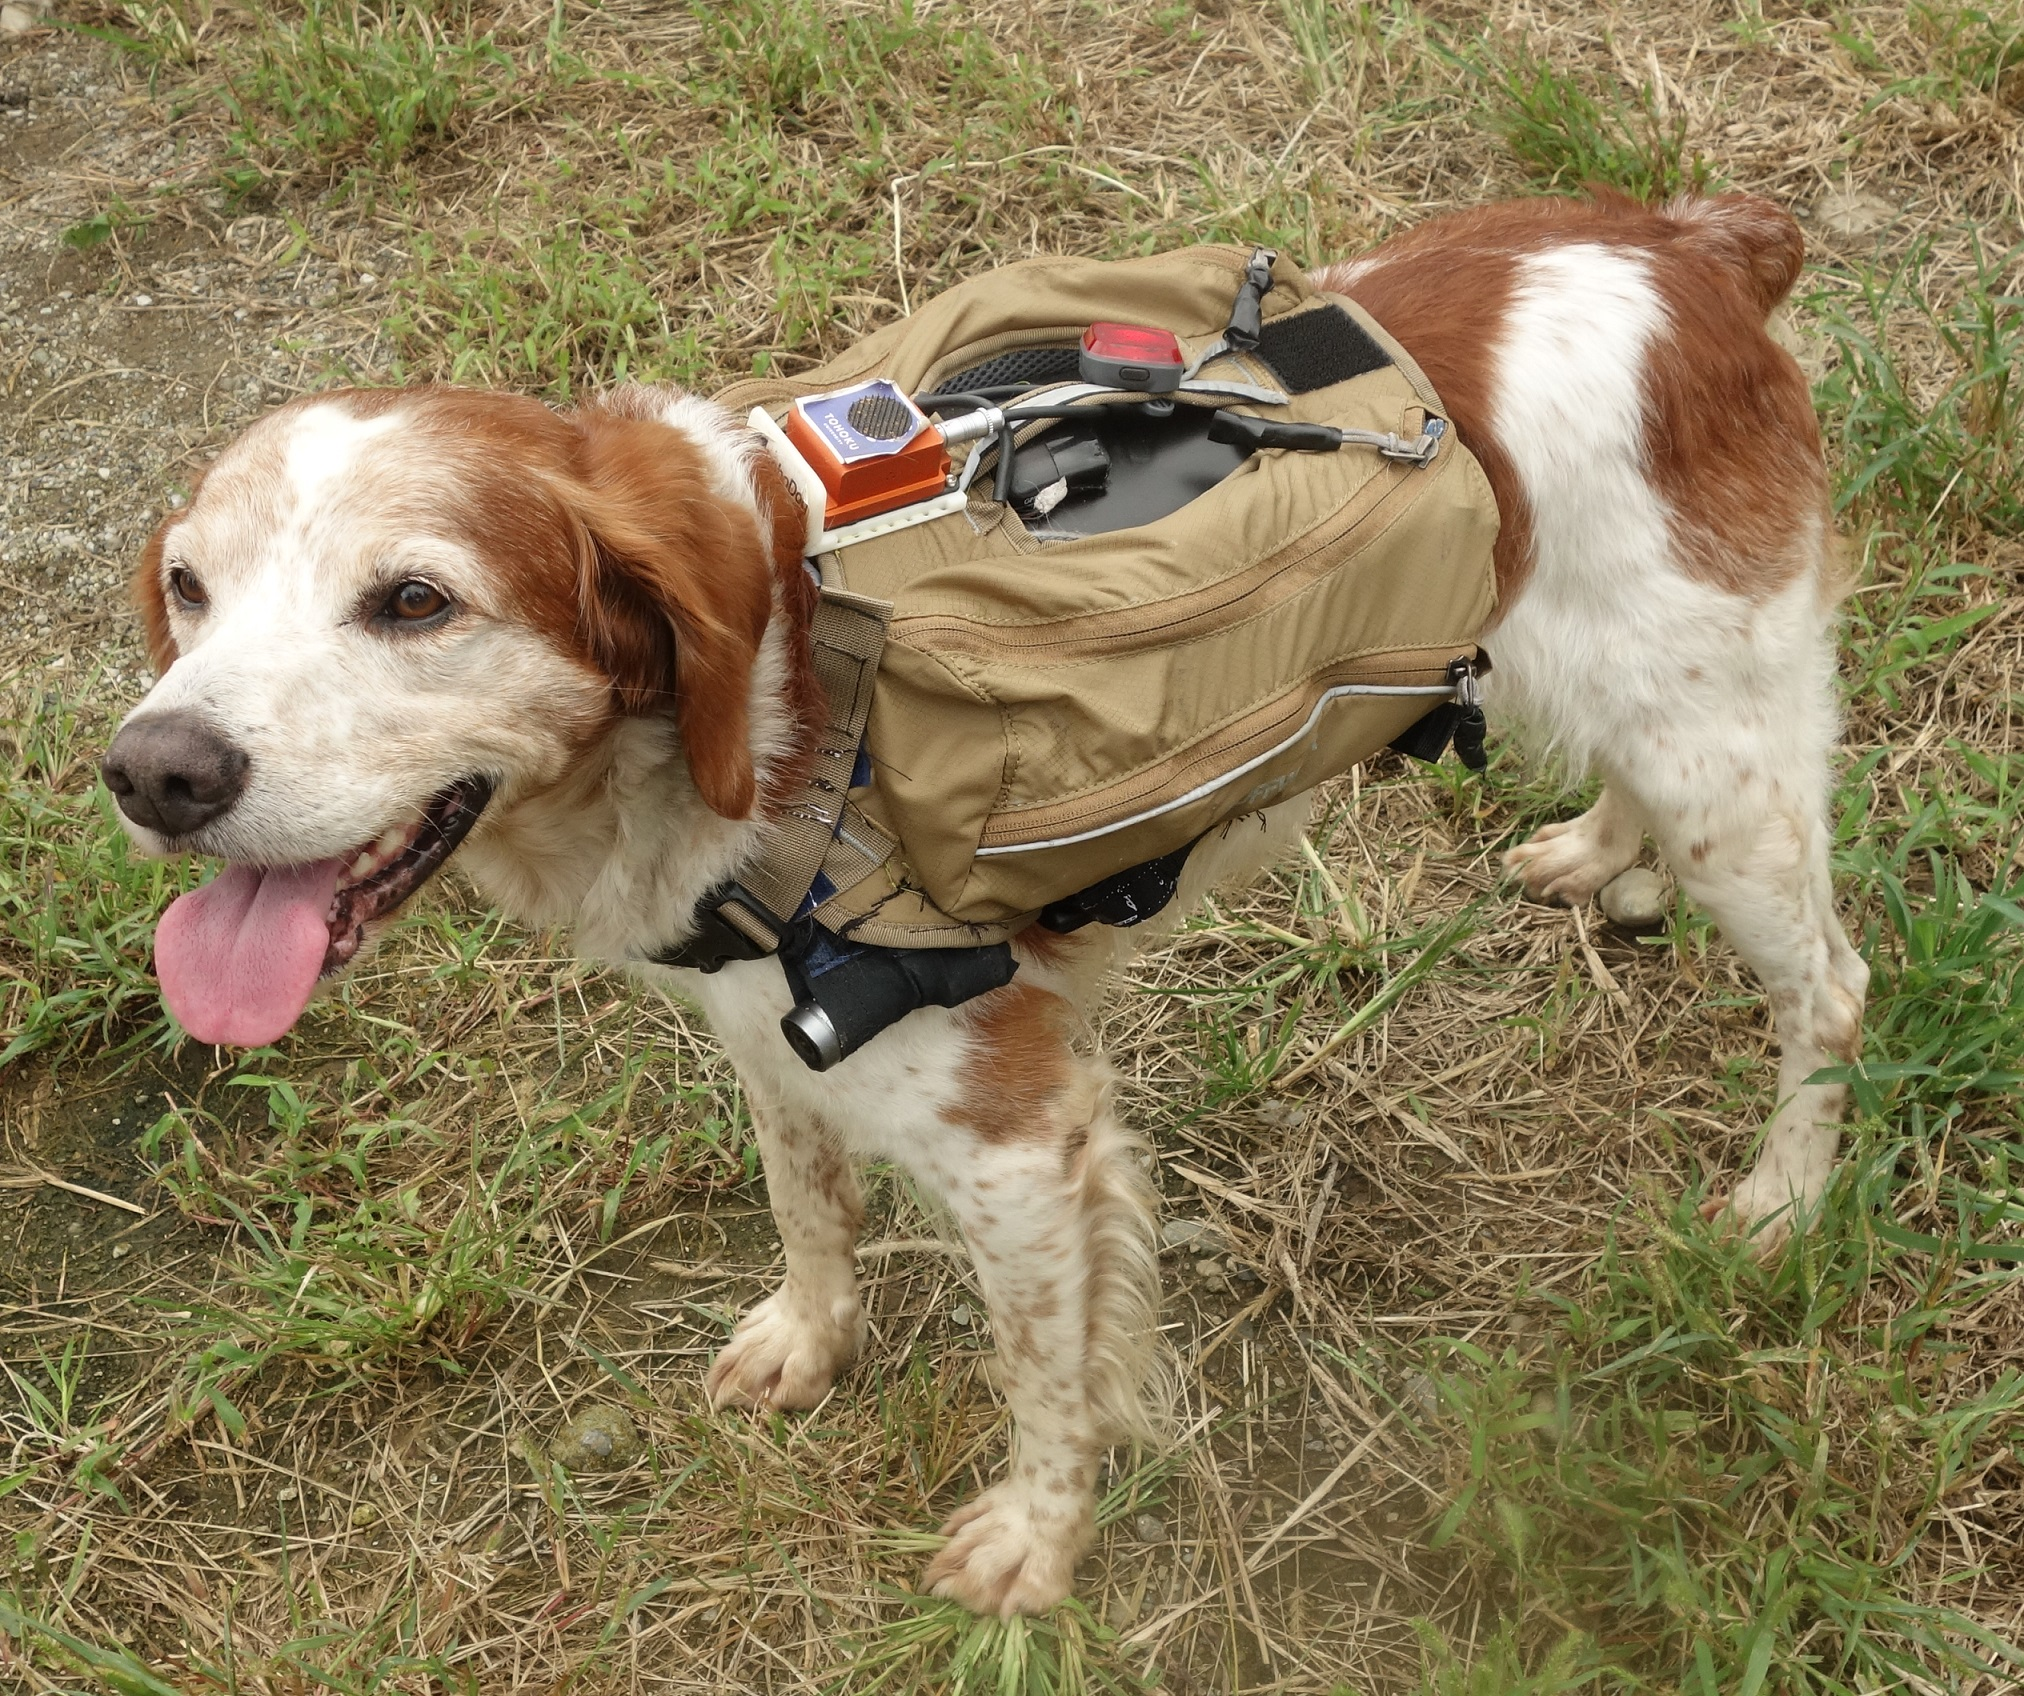
\includegraphics[width=9cm]{./Figures/cyberdog.eps}
%  \caption{装着型計測・記録装置~\cite{dog01}より引用}
%  \label{cyberdog}
% \end{center}
%\end{figure}

\subsection{音声からのマルチクラス推定}
動画の音声データのみを用いてマルチクラス推定を行なった.
ネットワークは\cite{aytar2016soundnet}の音声分類ネットワークを参考に構成した.
メル周波数スペクトラム係数を用いて音声データから特徴を取り出し,その値をネットワークへの入力とした.
29.97fpsの動画31フレーム分の音声を48000Hzとして扱い,(20, 94)次元の入力を得た.
\subsubsection{1D Convolutional network}
図~\ref{sound_network}に示したネットワークの2D Convolutionレイヤを1D Convolutionレイヤに置き換えたネットワークを用いて推定を行なった.
推定制度を表~\ref{sound_1d_result}に示す.

全体を通して,静止画像からのマルチクラス推定よりも精度が上昇した.
特に,barkクラス,commandクラス,shakeクラス,sniffクラスの精度上昇が顕著であり,音特徴がクラス推定に重要であることが示された.
\begin{table}[tb]
 \centering
 \caption{音声データを用いた1d Convolutional networkの推定結果}\label{sound_1d_result}
 \scalebox{0.80}[0.80]{
  \begin{tabular}{|l||c|c|c|c|c|c|c|c|c|c|c|c|}
   \hline \hline
   クラス   & \rotatebox{90}{bark}& \rotatebox{90}{cling}&\rotatebox{90}{command}& \rotatebox{90}{eat}&\rotatebox{90}{handler}& \rotatebox{90}{run}&\rotatebox{90}{victim}& \rotatebox{90}{shake}& \rotatebox{90}{sniff}& \rotatebox{90}{stop}& \rotatebox{90}{walk} & \rotatebox{90}{全体}\\ \hline

   %seven80_6fps_sound_bc-128_lr-4_1d
Precision & 0.909& 0.13& 0.361& 0.141& 0.245& 0.0& 0.419& 0.708& 0.583& 0.919& 0.759&  0.699 \\ \hline
Recall    & 0.717& 0.161& 0.361& 0.026& 0.24& 0.0& 0.442& 0.538& 0.781& 0.798& 0.907&  0.656 \\ \hline
Jaccard   & 0.669& 0.078& 0.22& 0.023& 0.138& 0.0& 0.274& 0.44& 0.502& 0.745& 0.704&  0.512 \\ \hline


  \end{tabular}
 }
\end{table}

\subsubsection{2D Convolutional network}
音声データから得た(20, 94)次元の入力にチャネルを追加し,(1, 20, 94)の画像としてネットワークへ入力した.
1D Convolutional networkと比較し特徴量が増えたが,全体での精度には大きな差は出なかった.
推定精度を表~\ref{sound_2d_label}に示す.
学習コストなどを含めるなど評価指標を変えた際には2D Convolutional networkが劣る部分がある.
\begin{table}[tb]
 \centering
 \caption{音声データを用いた2d Convolutional networkの推定結果}\label{sound_2d_result}
 \scalebox{0.80}[0.80]{
  \begin{tabular}{|l||c|c|c|c|c|c|c|c|c|c|c|c|}
   \hline \hline
   クラス   & \rotatebox{90}{bark}& \rotatebox{90}{cling}&\rotatebox{90}{command}& \rotatebox{90}{eat}&\rotatebox{90}{handler}& \rotatebox{90}{run}&\rotatebox{90}{victim}& \rotatebox{90}{shake}& \rotatebox{90}{sniff}& \rotatebox{90}{stop}& \rotatebox{90}{walk} & \rotatebox{90}{全体}\\ \hline
Precision & 0.844& 0.094& 0.357& 0.013& 0.192& nan& 0.407& 0.794& 0.588& 0.917& 0.808&  0.639 \\ \hline
Recall    & 0.628& 0.064& 0.285& 0.002& 0.079& 0.0& 0.284& 0.33& 0.83& 0.797& 0.898&  0.721 \\ \hline
Jaccard   & 0.563& 0.04& 0.188& 0.001& 0.059& 0.0& 0.201& 0.304& 0.524& 0.744& 0.74&  0.512 \\ \hline


   % seven80_6fps_sound_bc-64_lr-0
%Precision & 0.86& 0.116& 0.243& 0.032& 0.194& 0.0& 0.375& 0.733& 0.565& 0.909& 0.766&  0.65 \\ \hline
   %Recall & 0.754& 0.333& 0.226& 0.006& 0.128& 0.0& 0.48& 0.524& 0.824& 0.742& 0.867&  0.642 \\ \hline
   %Jaccard & 0.672& 0.094& 0.133& 0.005& 0.083& 0.0& 0.267& 0.44& 0.504& 0.691& 0.686&  0.477 \\ \hline

  \end{tabular}
 }
\end{table}

\subsection{Two-stream network}
静止画像とoptical flow画像を学習していないVGG16ネットワークにそれぞれ入力し,得られた2つの出力を結合した結果からマルチクラス推定を行なった.
推定結果を表~\ref{stilloptic_result}に示す.

静止画像単体,optical flow画像単体からの推定と比較して精度がわずかに上昇している.
特にsniffクラスなどが劇的に精度が上昇している.動画から得られた静止画像の画像特徴に加えて,optical flowから得られる動き特徴をそれぞれ用いた学習ができていると考えられる.
ただし,shakeクラスなど,静止画像とoptical flow画像がお互いに悪影響を与え全く分類できなくなってしまったクラスも存在している.
\begin{table}[tb]
 \centering
 \caption{Two-stream networkの推定結果}\label{stilloptic_result}
 \scalebox{0.85}[0.85]{
  \begin{tabular}{|l||c|c|c|c|c|c|c|c|c|c|c|c|}
   \hline \hline
   クラス   & \rotatebox{90}{bark}& \rotatebox{90}{cling}&\rotatebox{90}{command}& \rotatebox{90}{eat}&\rotatebox{90}{handler}& \rotatebox{90}{run}&\rotatebox{90}{victim}& \rotatebox{90}{shake}& \rotatebox{90}{sniff}& \rotatebox{90}{stop}& \rotatebox{90}{walk} & \rotatebox{90}{全体}\\ \hline
Precision & 0.522& 0.04& 0.315& 0.0& 0.395& nan& 0.478& nan& 0.472& 0.848& 0.771&  0.571 \\ \hline
Recall    & 0.122& 0.033& 0.047& 0.0& 0.204& 0.0& 0.36& 0.0& 0.813& 0.807& 0.833&  0.646 \\ \hline
Jaccard   & 0.11& 0.018& 0.043& 0.0& 0.155& 0.0& 0.259& 0.0& 0.426& 0.705& 0.668&  0.435 \\ \hline

   % seven80_6fps_stilloptic_bc-128_lr-0_sr-5_sp-20

  \end{tabular}
 }
\end{table}

\subsection{Sound based Two-stream network}
音声データに静止画像,optical flow画像を個別に組み合わせ,マルチクラス推定を行なった.
音声の特徴を取り出すネットワークには2D Convolutional networkを用いた.
\subsubsection{音声データと静止画像からのマルチクラス推定}
音声と静止画像を組み合わせたマルチクラス推定の結果を表~\ref{stillsound_result}に示す.
静止画像単体と比較すると精度が上昇しているが,音声単体と比べると精度が下がっている.
クラス別で精度の比較をした際に、唯一see victimクラスの精度が上昇している.
基本的に精度が低い静止画像単体でのマルチクラス推定の結果の中では,barkクラス,see victimクラスがやや精度が良い.
see victimクラスは,要救助者を発見して吠えている音声情報に加え,被災者がカメラに高頻度で映っている.
Recallについて静止画像の数値が高いことからも,音声と静止画像が不足する情報を互いに補い合ったため精度が上昇したことが推察できる.
barkクラスは音の情報の重要度が高いことが推測されるため,静止画像と音声を合わせての精度の上昇が認められなかったのではないだろうか.

ただし,実験に用いた音声用ストリームはConv2Dである.Conv2Dの音声ストリームを単体で用いた結果と音声と静止画像を入力とした結果をクラス別に比較すると,クラスによっては精度が上昇しているものもある.
以下Conv1Dの結果を除き,静止画像での学習結果,Conv2D音声ストリームでの学習結果,静止画像とConv2D音声ストリームを合わせた学習結果について考察する.

全体としては音声単体の方が精度が高かった.
しかし,see victimクラスの精度が顕著に上昇したように,静止画像ストリームが悪影響を与えているとは断言できない.
それぞれの単体での結果よりも精度の上昇したクラスはbark,command,handler,run,see victim,shakeクラスである.
静止画像単体の方が精度が高いクラスはcling,eatクラスであり,
Conv2D音声ストリーム単体の方が精度が高いクラスはsniff,stop,walkクラスである.
静止画像単体で精度の高いクラスは,画像に特徴が現れやすいクラスであり,人間が識別するにも音声を重要としない.
音声単体で精度の高い3クラスは動画として見る際には人間にも識別しやすいが,静止画像とするとやや難解である.時間情報を含む音声の方が特徴が現れやすいと言える.また,データ数が特に多い点も共通している.
組み合わせた結果で精度の上昇したクラスに共通している点は,人間に音と画像の両情報から識別が可能であるか,あるいは場合によってどちらの情報を重視して判断するかが変わる点である.
これらを踏まえると,音声と静止画像を組み合わせてのマルチラベル推定は両単体での推定精度を超えることが期待できる.

\begin{table}[tb]
 \centering
 \caption{音声と静止画像からのマルチクラス推定結果}\label{stillsound_result}
 \scalebox{0.75}[0.75]{
  \begin{tabular}{|l||c|c|c|c|c|c|c|c|c|c|c|c|}
   \hline \hline
   クラス   & \rotatebox{90}{bark}& \rotatebox{90}{cling}&\rotatebox{90}{command}& \rotatebox{90}{eat}&\rotatebox{90}{handler}& \rotatebox{90}{run}&\rotatebox{90}{victim}& \rotatebox{90}{shake}& \rotatebox{90}{sniff}& \rotatebox{90}{stop}& \rotatebox{90}{walk} & \rotatebox{90}{全体}\\ \hline
  Precision & 0.909& 0.05& 0.312& 0.051& 0.249& 0.042& 0.42& 0.56& 0.592& 0.885& 0.787&  0.661 \\ \hline
Recall    & 0.709& 0.077& 0.341& 0.028& 0.177& 0.002& 0.537& 0.589& 0.758& 0.802& 0.855&  0.673 \\ \hline
Jaccard   & 0.662& 0.031& 0.195& 0.018& 0.115& 0.002& 0.308& 0.402& 0.498& 0.726& 0.694&  0.5 \\ \hline


   %seven80_6fps_stillsound_bc-32_lr-05
  \end{tabular}
 }
\end{table}

\subsubsection{音声データとoptidcal flow画像からのマルチクラス推定}
音声とoptical flow画像を組み合わせたマルチクラス推定の結果を表~\ref{opticsound_result}に示す.
静止画像単体,optical flow画像単体,静止画像とoptical flowのTwo-streamと比較して精度は上がったが,音声を用いた結果それぞれと比較すると精度は下がったと言える.
基本的には前項で述べた比較と同じである.そのため前項との差分についてのみ述べる.

顕著に精度の上がったクラスはcommand,stopクラスである.本研究の実験を通して最もcommandクラスの精度が高かった.
stopクラスについては図~\ref{cyberdataset_img}に示したoptical flow画像と静止画像,音声を比較すると,そのoptical flow画像の特徴は歴然である.
これがoptical flow画像を用いてstopクラスの精度が上昇した理由と言える.
データセットには基本的にwalkかstopのクラスがついていることも考慮し,walk,stopクラスのPrecisionとRecallを比較するとstopクラス検知数の増加がwalkクラス検知数の減少に繋がっていることが読み取れる.
stopクラスのPredcisionが下がり,誤検知が増えている.これは,walkクラスをstopクラスと認識していると考えられる.
この考察から期待される結果は,walkクラスのPrecisionの上昇であるが,walkクラスはPrecisionもRecallも減少している.
stopクラスが特徴的であるのに対し,walkクラスには様々なパターンが存在する.むしろ,レスキュー犬が動くことによる画像のブレやボケの特徴が失われている.
そのため,stopクラスを学習できてもwalkクラスの学習には繋がらなかったと考えられる.

静止画像と音声の識別と比較し,stopクラスと同様の理由で逆に精度が下がったクラスがsee victimクラスである.
レスキュー犬は要救助者を発見すると基本的にその場に停止する.optical flow画像の動き情報からsee victimクラスの特徴は得られないのである.

\begin{table}[tb]
 \centering
 \caption{音声とoptical flow画像からのマルチクラス推定結果}\label{opticsound_result}
 \scalebox{0.75}[0.75]{
  \begin{tabular}{|l||c|c|c|c|c|c|c|c|c|c|c|c|}
   \hline \hline
   クラス   & \rotatebox{90}{bark}& \rotatebox{90}{cling}&\rotatebox{90}{command}& \rotatebox{90}{eat}&\rotatebox{90}{handler}& \rotatebox{90}{run}&\rotatebox{90}{victim}& \rotatebox{90}{shake}& \rotatebox{90}{sniff}& \rotatebox{90}{stop}& \rotatebox{90}{walk} & \rotatebox{90}{全体}\\ \hline
Precision & 0.887& 0.071& 0.332& 0.052& 0.245& 0.143& 0.329& 0.692& 0.564& 0.881& 0.791&  0.681 \\ \hline
Recall    & 0.729& 0.177& 0.441& 0.019& 0.198& 0.01& 0.409& 0.424& 0.782& 0.845& 0.847&  0.641 \\ \hline
Jaccard   & 0.667& 0.054& 0.234& 0.014& 0.123& 0.01& 0.223& 0.356& 0.487& 0.759& 0.692&  0.493 \\ \hline

%seven80_6fps_opticsound_bc-64_lr-0
  \end{tabular}
 }
\end{table}

\subsection{Sound based Three-stream network}
静止画像・optical flow画像・音声を用いてSound based Three-streamでレスキュー犬行動のマルチラベル推定を行なった.
結果を表~\ref{stillopticsound_result}に示す.

音声単体,Sound based Two-streamと比較して精度が上昇した.
3つのデータから得られた特徴が民主主義的に出力を得るため,どれか1つのストリームが誤った推定をしても他2つがカバーしていると考えられる.
当初期待した,お互いがお互いの不足する情報を補い合った結果が得られた.
2つの入力だった場合とは異なり,信頼できる結果は尊重しあい,足を引っ張り合うケースが減り全体の精度上昇に繋がった.

\begin{table}[tb]
 \centering
 \caption{静止画像とoptical flow画像と音声からのマルチクラス推定結果}\label{stillopticsound_result}
 \scalebox{0.75}[0.75]{
  \begin{tabular}{|l||c|c|c|c|c|c|c|c|c|c|c|c|}
   \hline \hline
   クラス   & \rotatebox{90}{bark}& \rotatebox{90}{cling}&\rotatebox{90}{command}& \rotatebox{90}{eat}&\rotatebox{90}{handler}& \rotatebox{90}{run}&\rotatebox{90}{victim}& \rotatebox{90}{shake}& \rotatebox{90}{sniff}& \rotatebox{90}{stop}& \rotatebox{90}{walk} & \rotatebox{90}{全体}\\ \hline
Precision & 0.888& 0.165& 0.282& 0.188& 0.313& 0.212& 0.527& 0.708& 0.621& 0.891& 0.822&  0.702 \\ \hline
Recall    & 0.623& 0.423& 0.355& 0.092& 0.306& 0.029& 0.709& 0.492& 0.783& 0.861& 0.86&  0.663 \\ \hline
Jaccard   & 0.577& 0.135& 0.186& 0.066& 0.183& 0.026& 0.433& 0.409& 0.53& 0.779& 0.725&  0.518 \\ \hline


%seven80_6fps_stillopticsound_bc-128_lr-0
  \end{tabular}
 }
\end{table}
